\documentclass[11pt]{article}
\usepackage[margin=0.85in]{geometry}
\usepackage{amsmath,booktabs,graphicx,hyperref,listings,enumitem,float}
\graphicspath{{figures/}}
\hypersetup{colorlinks=true,urlcolor=blue}
\setlist{nosep,leftmargin=*}
\lstset{basicstyle=\ttfamily\footnotesize,breaklines=true,frame=single,columns=fullflexible}

\title{CS 839 Programming Assignment\\Sustained Two-Leg Support for MuJoCo Ant}
\author{Haoyang Tang}
\date{Fall 2026}

\begin{document}
\maketitle

\section{Interesting Behavior}
The Ant should remain upright with exactly two feet on the ground for as much
of each episode as possible. Balancing this unstable body using eight joint
torques, without support from another foot or body part, is non-trivial.

\section{Task MDP}
\begin{description}[style=nextline]
\item[State.] A 118-dimensional vector: the standard Ant joint, velocity, and
contact-force observation, plus four foot-contact indicators, normalized target
hold progress, and a two-element target-pair indicator.
\item[Action.] Eight continuous joint torques in $[-1,1]^8$.
\item[Reward.] Let $I_t$ mark a valid two-leg pose, $h_t$ and $u_t$ be clipped
height and upright scores, $d_t$ target-contact quality, $p_t$ hold progress,
$b_t$ a completed target hold, $B_t$ body contact, and $D_t$ termination:
\[
r_t=c_t+h_t+u_t+4I_t+0.5d_th_tu_t+2p_t+2b_t
-4B_t-0.02\lVert\omega_t\rVert^2-0.02\lVert a_t\rVert^2-20D_t,
\]
where $c_t=\max(0,1-0.5|n_t-2|)$ and $n_t$ is the number of grounded feet.
\item[Episode.] 1,000 steps at $0.05$ seconds per step, or 50 seconds.
\item[Termination.] Terminate if torso up-alignment is below $-0.2$ or the
simulation becomes non-finite; otherwise truncate at 1,000 steps.
\end{description}
The observation includes the mechanical state and reward-relevant task memory,
so I treat it as Markov for this position-invariant task.

\section{True Performance Metric}
A valid pose has exactly two grounded feet, torso height at least $0.45$ m,
positive torso up-alignment, and no other body contact. Performance is
\[
M=0.05\sum_{t=1}^{T}\mathbf{1}[\text{valid two-leg pose at }t],
\]
measured in seconds from 0 to 50. It directly measures the intended behavior
and excludes reward-shaping terms.

\section{Training Performance}
I used paired training seeds 1--5. I smoothed each seed with a 20-episode
rolling mean, interpolated it onto a 5,000-step grid, and then averaged. Thin
lines are individual seeds; shading is the 95\% Student-$t$ interval
$\bar{x}\pm2.776s/\sqrt{5}$.

\begin{figure}[H]
\centering
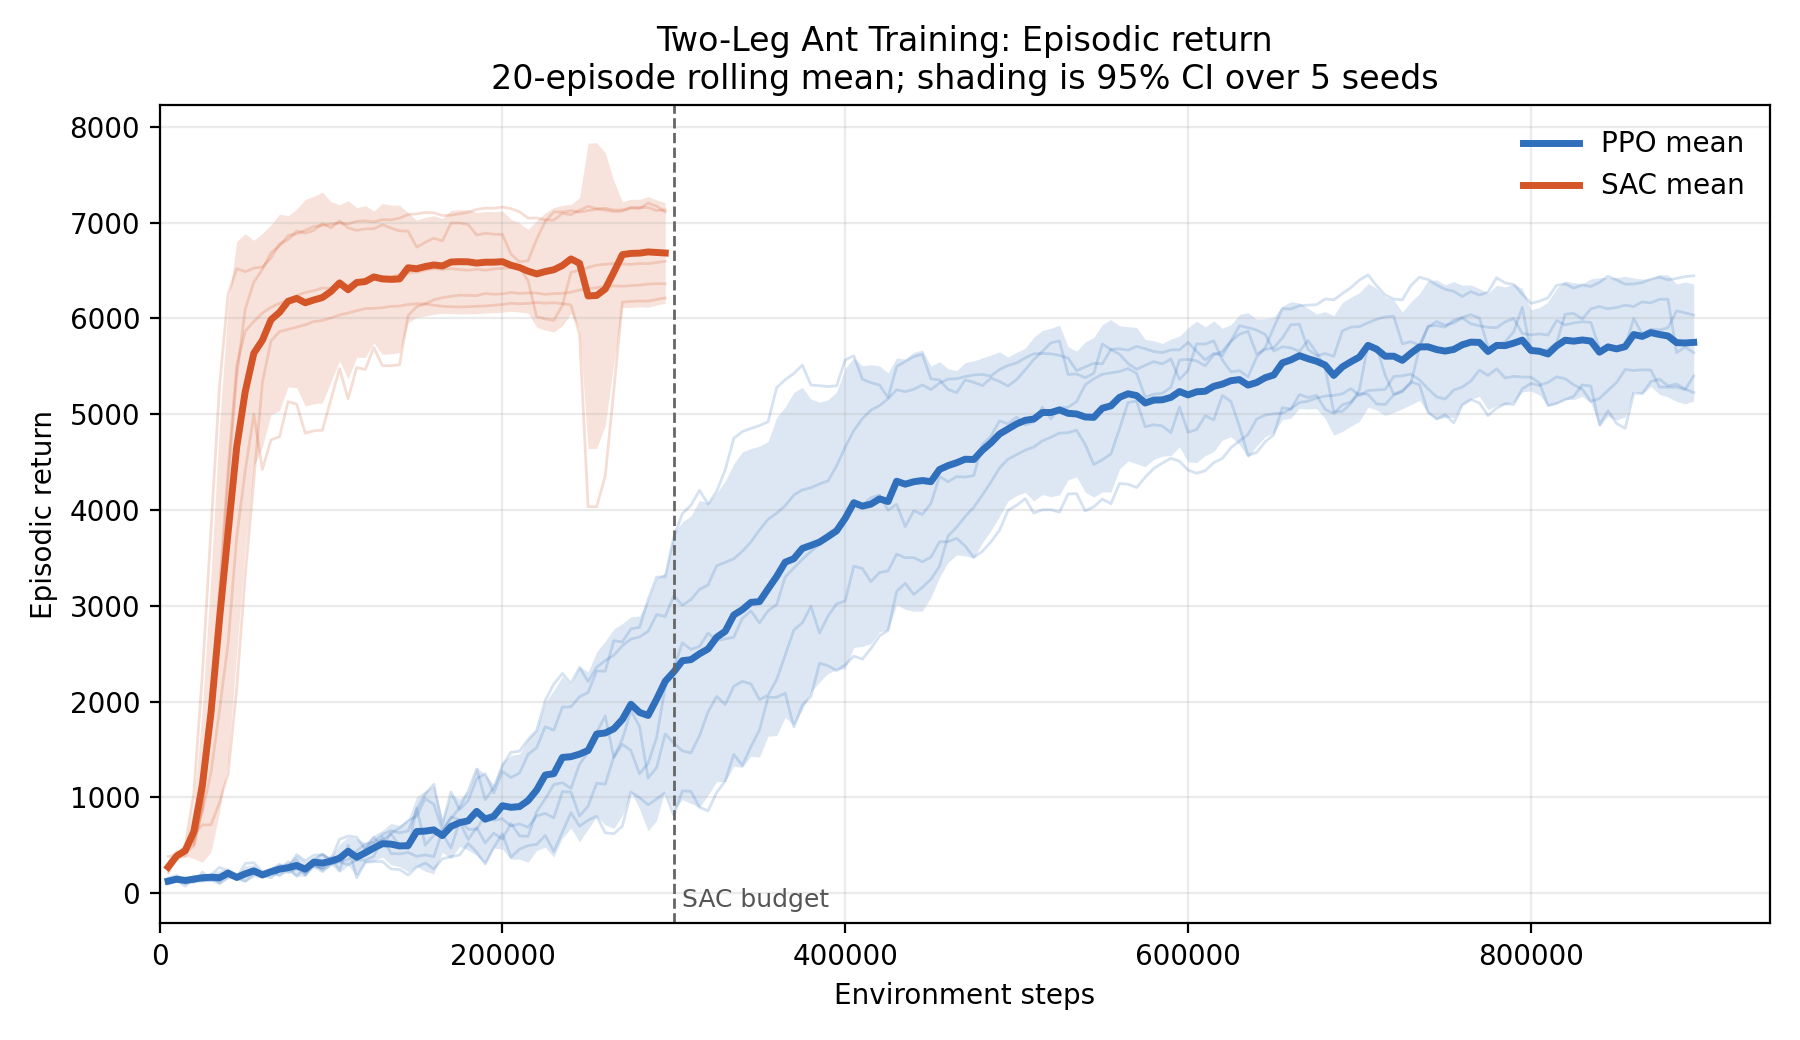
\includegraphics[height=0.29\textheight]{training_return.png}
\caption{Mean episodic return. SAC ends at 300,000 steps; PPO continues to
approximately 899,000 steps.}
\end{figure}

\begin{figure}[H]
\centering
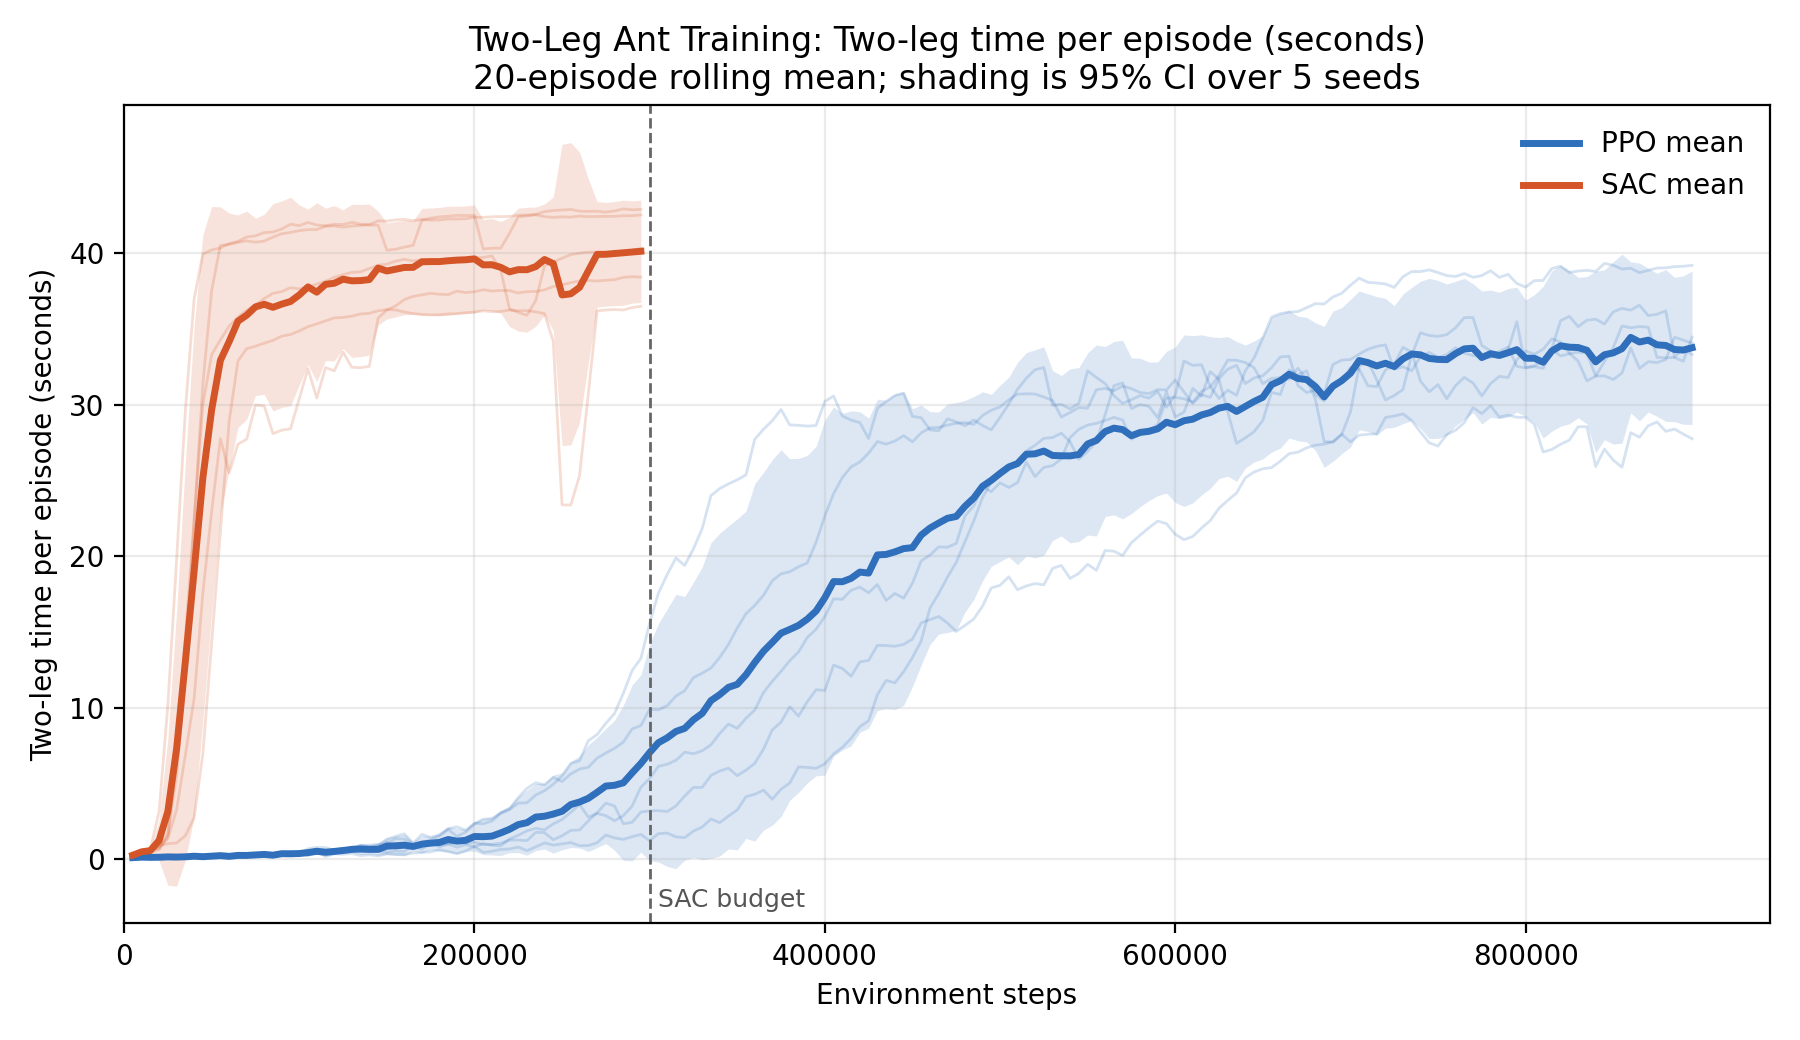
\includegraphics[height=0.29\textheight]{training_true_performance.png}
\caption{Mean true performance: valid two-leg seconds per 50-second episode.}
\end{figure}

\section{Algorithm Comparison}
Final deterministic evaluation used the same ten evaluation seeds for every
policy. Values are means and 95\% intervals across five training seeds.

\begin{table}[H]
\centering
\small
\begin{tabular}{lrrrr}
\toprule
 & Return & Two-leg time (s) & Fraction & Longest hold (s) \\
\midrule
PPO & $6011\pm386$ & $36.11\pm3.58$ & $0.722\pm0.072$ & $0.969\pm0.539$ \\
SAC & $6777\pm571$ & $40.66\pm3.09$ & $0.813\pm0.062$ & $1.111\pm0.287$ \\
\bottomrule
\end{tabular}
\end{table}

SAC achieved higher observed final performance despite using 300,000 steps,
versus 899,072 for PPO. Its smoothed mean exceeded 35 two-leg seconds near
65,000 steps; PPO first exceeded 30 seconds near 645,000 steps. SAC was likely
more sample-efficient because its replay buffer reuses experience, while PPO is
on-policy. True-metric standard deviation was 2.49 s for SAC and 2.89 s for PPO,
although SAC's return varied more. The paired SAC improvement in two-leg time
was $4.55$ s with a 95\% interval of $[-1.34,10.44]$, so it is not conclusive
with five seeds.

Earlier survival, height, sparse-bonus, and alternating-pair rewards produced
upright motion or preference for one pair rather than reliable two-foot
support. Dense valid-pose and hold-progress rewards improved total two-leg time.
However, all final policies recorded zero valid pair switches and only about a
one-second longest continuous hold. They solve aggregate two-leg time, not the
more ambitious alternating-pair behavior.

\section{Best Policy Video}
\texttt{best\_policy\_sac\_seed3.mp4} shows the best policy: SAC seed 3,
averaging 43.12 two-leg seconds (86.24\% of an episode). It stays upright but
does not alternate support pairs.

\section{Reproducibility}
Code is included and available at \url{https://github.com/Sacbill/839homework}.
Exact paired-run commands are:
\begin{lstlisting}[language=bash]
for seed in 1 2 3 4 5; do
  .venv/bin/python cleanrl/ppo_two_leg.py --env-id AntTwoLeg-v0 \
    --exp-name ppo_sustained_hold_v4 --seed "$seed" \
    --total-timesteps 900000 --eval-episodes 10 --capture-video --save-model
done
for seed in 1 2 3 4 5; do
  .venv/bin/python cleanrl/sac_two_leg.py --env-id AntTwoLeg-v0 \
    --exp-name sac_sustained_hold_v4 --seed "$seed" \
    --total-timesteps 300000 --learning-starts 5000 --buffer-size 300000 \
    --eval-episodes 10 --capture-video --save-model
done
.venv/bin/python analysis/two_leg_five_seed/analyze_runs.py
\end{lstlisting}

\section*{AI Use Disclosure}
I used OpenAI Codex for reward-design discussion, implementation and debugging
assistance, result analysis, plotting, and report preparation. I reviewed the
experiments and take responsibility for the submitted work.

\end{document}
